\documentclass{beamer}

\usepackage{pres}

\title{\trtitle}
\author{\trauthor}
\date{\trdate}

\begin{document}

\frame{\titlepage}

\begin{frame}
  \frametitle{Background}

  \begin{columns}
    \begin{column}{.7\linewidth}
      \begin{itemize}
        \item Bachelor 
        \item NLP
      \end{itemize}
    \end{column}

    \begin{column}{.2\linewidth}
      
\includegraphics[width=.9\linewidth]{tsinghua}
    \end{column}
  \end{columns}

  ~

  \begin{columns}
    \begin{column}{.6\linewidth}
      \begin{itemize}
        \item Master
        \item CINACS - Crossmodal Interaction in Natural and Artificial Cognitive Systems
      \end{itemize}
    \end{column}

    \begin{column}{.3\linewidth}
      
\includegraphics[width=.9\linewidth]{uhh}
    \end{column}
  \end{columns}
\end{frame}

\frame{
  \frametitle{Outline}
  \tableofcontents
}

\section{Introduction}
\begin{frame}
  \frametitle{Motivation}

  \begin{itemize}
    \item Human use multiple sensory information to recognize objects.

      ~
    \item Difficulties of visual object recognition:
      \begin{itemize}
        \item Sensitive to image transformations. 
      \end{itemize}

      ~
    \item Sound provides complementary information.
      \begin{itemize}
        \item Make sound via interactions.
        \item Information about material. 
        \item Category by function: objects that make sound.
      \end{itemize}
  \end{itemize}
\end{frame}

\begin{frame}
  \frametitle{Related Work}

  \begin{itemize}
    \item Sinapov and his colleagues~\cite{sinapov_interactive_2009,sinapov_object_2011}: 
      \begin{itemize}
        \item Audio and proprioceptive information.
        \item Relational learning.

          ~
        \item No visual information.
      \end{itemize}

      ~
    \item Nakamura and his colleagues~\cite{nakamura_multimodal_2007,nakamura_bag_2012}:
      \begin{itemize}
        \item Visual, audio and haptic information.
        \item Multimodal pLSA.

          ~
        \item Unsupervised categorization.
      \end{itemize}
  \end{itemize}
\end{frame}

\begin{frame}
  \frametitle{Objective}

  \begin{itemize}
    \item Build an object recognition system based on visual and audio information.

      ~
      \begin{itemize}
        \item What kind of features?

          ~
        \item How to make classification?

          ~
        \item How to combine multimodal information?
      \end{itemize}
  \end{itemize}
\end{frame}

\iffalse
\begin{frame}
  \frametitle{Two Tasks of Object Recognition}

  \begin{itemize}
    \item Specific object recognition.
      \includegraphics[width=\linewidth]{specific.tikz}

    \item Generic category recognition.
      \includegraphics[width=\linewidth]{generic.tikz}
  \end{itemize}
\end{frame}
\fi

\section{Feature Extraction}
\iffalse
\begin{frame}
  \frametitle{Bag-of-Words Model with SIFT Descriptors}

  \begin{itemize}
    \item SIFT Descriptor~\cite{lowe_object_1999}. 
      \begin{itemize}
        \item Local feature descriptor invariant to several image transforms.
        \item Standard for object recognition in robotics.

          ~
        \item Does not describe the whole image/object.
        \item Does not encode general features of a category.
      \end{itemize}
  \end{itemize}

  \centering
  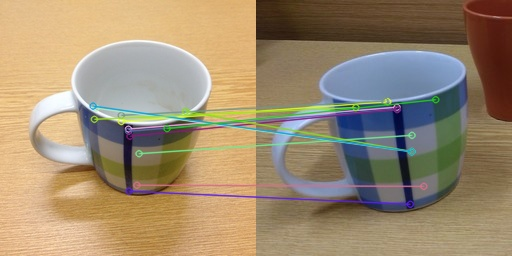
\includegraphics[width=.7\linewidth]{mug2m}
\end{frame}
\fi

\begin{frame}
  \frametitle{Bag-of-Words Model with SIFT Descriptors}

  \begin{columns}
    \begin{column}{.46\linewidth}
      \begin{itemize}
        \item Bag-of-words model. 
        \item An image : a collection of local features.
      \end{itemize}
      \centering
      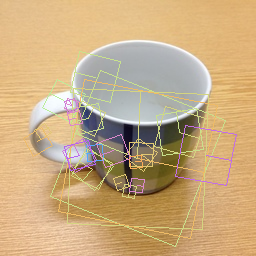
\includegraphics[width=.5\columnwidth]{mug2k}
    \end{column}

    \begin{column}{.46\linewidth}
      \begin{itemize}
        \item Vector quantization with a codebook.
          \begin{itemize}
            \item
              
\includegraphics[width=.1\columnwidth]{mug2v11}~ : 1
            \item
              
\includegraphics[width=.1\columnwidth]{mug2v21}~
              
\includegraphics[width=.1\columnwidth]{mug2v22}~
              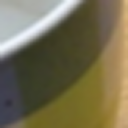
\includegraphics[width=.1\columnwidth]{mug2v23}~ : 3
            \item
              
\includegraphics[width=.1\columnwidth]{mug2v31}~
              
\includegraphics[width=.1\columnwidth]{mug2v32}~
              
\includegraphics[width=.1\columnwidth]{mug2v33}~ : 3
            \item
              
\includegraphics[width=.1\columnwidth]{mug2v41}~
              
\includegraphics[width=.1\columnwidth]{mug2v42}~ : 2
            \item \ldots
          \end{itemize}
      \end{itemize}
    \end{column}
  \end{columns}
\end{frame}

\begin{frame}
  \frametitle{Mel-frequency Cepstrum Coefficients}

  \begin{itemize}
    \item DCT of log power spectrum at mel-scale.

      ~
    \item MFCCs are common acoustic features for audio processing, such as speech recognition and speaker recognition.
  \end{itemize}
\end{frame}

\section{Hidden Markov Models}
\begin{frame}
  \frametitle{Hidden Markov Models}

  \begin{itemize}
    \item During interactions images and sound change over time.
    \item HMM describes a distribution of a stochastic process.
      \begin{itemize}
        \item Applications in many fields including speech recognition, gesture recognition and so on. 
      \end{itemize}
      ~

    \item HMM is a generative model.
      \begin{itemize}
        \item Allows further inference for modality fusion. 
      \end{itemize}
  \end{itemize}
\end{frame}

\begin{frame}
  \frametitle{Classification with HMM}

  \begin{itemize}
    \item Estimate $\lambda^c$ with all data of class $c$.

    \item Approximate likelihood with learned model:
      \[ P(\mathbf{x}|c) = P(\mathbf{x}|\lambda^c) . \]
    \item Specific object recognition (multiclass classification):
      \[ f(\mathbf{x}) = \argmax_{c} P(\mathbf{x}|c) \]
    \item Generic category recognition (binary classification):
      \[ 
        f(\mathbf{x}) = \left\{
          \begin{array}{l l}
            +1, & \quad P(c=+1|\mathbf{x}) > \theta; \\
            -1, & \quad \text{otherwise.}
          \end{array} \right.
        \]
        where
        \[ P(c|\mathbf{x}) = \frac{P(\mathbf{x}|c)P(c)}{\sum_{c \in \{-1,+1\}} P(\mathbf{x}|c)P(c)} . \]
    \end{itemize}
  \end{frame}

  \section{Bimodal Object Recognition}
  \begin{frame}
    \frametitle{Multimodal Fusion Methods}

    \begin{itemize}
      \item $\mathbf{x} = (\mathbf{v},\mathbf{a})$.
      \item The goal is to compute the joint likelihood:
        \[ P(\mathbf{v},\mathbf{a}|c) \]

        ~
      \item Two approaches:
        \begin{itemize}
          \item Feature Fusion.
          \item Decision Fusion.
        \end{itemize}
    \end{itemize}
  \end{frame}


  \begin{frame}
    \frametitle{Feature Fusion}

    \begin{center}
      \scriptsize
      \includegraphics[width=.9\linewidth]{featurefs.tikz}
    \end{center}

    \begin{itemize}
      \item Directly learn the joint likelihood with concatenated features:
        \[ P(\mathbf{v},\mathbf{a}|c) = P(\mathbf{v},\mathbf{a}|\lambda_{va}^c) \]
    \end{itemize}
  \end{frame}

  \begin{frame}
    \frametitle{Decision Fusion}

    \begin{center}
      \scriptsize
      \includegraphics[width=.9\linewidth]{decisionfs.tikz}
    \end{center}

    \begin{itemize}
      \item Learn separate models and combine them under conditional independence assumption:
        \[ P(\mathbf{v},\mathbf{a}|c) = P(\mathbf{v}|c) P(\mathbf{a}|c) = P(\mathbf{v}|\lambda_v^c) P(\mathbf{a}|\lambda_a^c) \]
    \end{itemize}
  \end{frame}

  \begin{frame}
    \frametitle{Comparison of Fusion Methods}

    \centering
    \begin{tabular}{p{.42\linewidth}|p{.42\linewidth}}
      \hline
      \multicolumn{1}{c|}{\bfseries Feature Fusion} & \multicolumn{1}{c}{\bfseries Decision Fusion} \\ \hline
      Theoretically correct. & Independent assumption needs to be hold. \\
      \\
      Models are complex. & Models are simple. \\
      \\
      Synchronization is \mbox{necessary}. & Synchronization is not necessary. \\ \hline
    \end{tabular}

  \end{frame}

  \section{Experiment}
  \begin{frame}
    \frametitle{Experiment Setup}

    \begin{columns}
      \begin{column}{.4\linewidth}
        \begin{itemize}
          \item 33 household objects.

            ~

          \item Interactions:
            \begin{itemize}
              \item Strike with a stick.
              \item Push.
              \item Shake.
            \end{itemize}
        \end{itemize}
      \end{column}
      \begin{column}{.55\linewidth}
        \begin{tabular}[t]{lc}
          \hline
          Mugs & \includegraphics[width=.14\linewidth]{object2} ~ 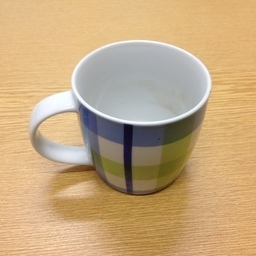
\includegraphics[width=.14\linewidth]{object3} ~ \includegraphics[width=.14\linewidth]{object6} \\
          Bottles & 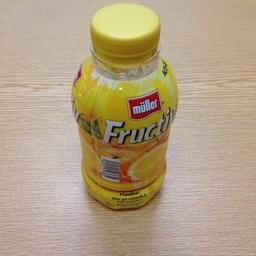
\includegraphics[width=.14\linewidth]{object16} ~ 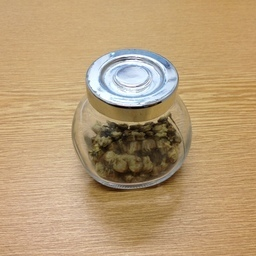
\includegraphics[width=.14\linewidth]{object19} ~ 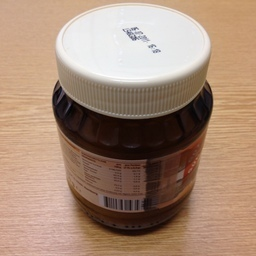
\includegraphics[width=.14\linewidth]{object20} \\
          Plastic & 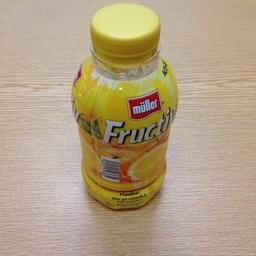
\includegraphics[width=.14\linewidth]{object16} ~ \includegraphics[width=.14\linewidth]{object17} ~ \includegraphics[width=.14\linewidth]{object33} \\
          Metal & \includegraphics[width=.14\linewidth]{object9} ~ \includegraphics[width=.14\linewidth]{object10} ~ \includegraphics[width=.14\linewidth]{object12} \\
          Fragile & \includegraphics[width=.14\linewidth]{object1} ~ \includegraphics[width=.14\linewidth]{object2} ~ \includegraphics[width=.14\linewidth]{object7} \\
          Containers & 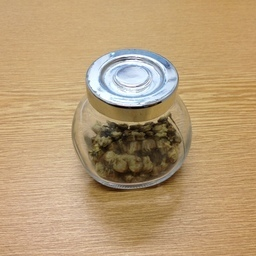
\includegraphics[width=.14\linewidth]{object19} ~ 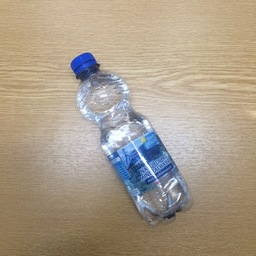
\includegraphics[width=.14\linewidth]{object24} ~ \includegraphics[width=.14\linewidth]{object29} \\
          \hline
        \end{tabular}
      \end{column}
    \end{columns}
  \end{frame}

  \begin{frame}
    \frametitle{Specific Object Recognition Result}

    \centering
    \begin{tabular}[h]{c|c}
      \hline
      Method & Accuracy \\ \hline \hline
      Feature Fusion & \textbf{95.8\%} \\ \hline
      Decision Fusion  & 95.7\% \\ \hline
      Visual Only & 86.7\% \\ \hline
      Audio Only & 83.6\% \\ \hline
    \end{tabular}

    ~
    \begin{itemize}
      \item 5-fold cross validation.
      \item HMM with 2 states, 6 mixture components and diagonal covariance matrix.
    \end{itemize}
    \vfill
    {\scriptsize
      \[ \text{accuracy} =  \frac{\text{\# correctly classified}}{\text{\# total}} \]
    }
  \end{frame}

  \iffalse
  \begin{frame}
    \frametitle{Generic Category Recognition Result}

    \begin{columns}
      \begin{column}{.5\linewidth}
        \centering
        \scriptsize
        \includegraphics[width=\columnwidth]{roc.tikz}
      \end{column}
      \begin{column}{.5\linewidth}
        \begin{itemize}
          \item Object-based cross validation.
          \item Receiver operating characteristic (ROC).
          \item Area under the curve (AUC).
            \begin{itemize}
              \item 0.5 => Random
              \item 1.0 => Perfect 
            \end{itemize}
        \end{itemize}
      \end{column}
    \end{columns}
    {\scriptsize
      \[ \text{true positive rate} =  \frac{\text{\# true positive}}{\text{\# conditional positive}} \]
      \[ \text{false positive rate} =  \frac{\text{\# false positive}}{\text{\# conditional negative}} \]
    }
  \end{frame}
  \fi

  \begin{frame}
    \frametitle{Generic Category Recognition Result}

    \begin{columns}
      \begin{column}{.6\linewidth}
        \centering
        \footnotesize
        \includegraphics[width=\columnwidth]{mug.tikz}
      \end{column}
      \begin{column}{.4\linewidth}
        \begin{itemize}
          \item Mugs
        \end{itemize}
        ~

        \footnotesize
        \begin{tabular}[h]{c|c}
          \hline
          Method & AUC \\ \hline \hline
          Feature Fusion & 0.750 \\ \hline
          Decision Fusion  & \textbf{0.771} \\ \hline
          Visual Only & 0.763 \\ \hline
          Audio Only & 0.642 \\ \hline
        \end{tabular}
      \end{column}
    \end{columns}
  \end{frame}

  \begin{frame}
    \frametitle{Generic Category Recognition Result}

    \begin{columns}
      \begin{column}{.6\linewidth}
        \centering
        \footnotesize
        \includegraphics[width=\columnwidth]{bottle.tikz}
      \end{column}
      \begin{column}{.4\linewidth}
        \begin{itemize}
          \item Bottles
        \end{itemize}
        ~

        \footnotesize
        \begin{tabular}[h]{c|c}
          \hline
          Method & AUC \\ \hline \hline
          Feature Fusion & \textbf{0.802} \\ \hline
          Decision Fusion  & 0.798 \\ \hline
          Visual Only & 0.778 \\ \hline
          Audio Only & 0.707 \\ \hline
        \end{tabular}
      \end{column}
    \end{columns}
  \end{frame}

  \begin{frame}
    \frametitle{Generic Category Recognition Result}

    \begin{columns}
      \begin{column}{.6\linewidth}
        \centering
        \footnotesize
        \includegraphics[width=\columnwidth]{plastic.tikz}
      \end{column}
      \begin{column}{.4\linewidth}
        \begin{itemize}
          \item Plastic objects
        \end{itemize}
        ~

        \footnotesize
        \begin{tabular}[h]{c|c}
          \hline
          Method & AUC \\ \hline \hline
          Feature Fusion & 0.820 \\ \hline
          Decision Fusion & \textbf{0.839} \\ \hline
          Visual Only & 0.813 \\ \hline
          Audio Only & 0.732 \\ \hline
        \end{tabular}
      \end{column}
    \end{columns}
  \end{frame}
  \begin{frame}
    \frametitle{Generic Category Recognition Result}

    \begin{columns}
      \begin{column}{.6\linewidth}
        \centering
        \footnotesize
        \includegraphics[width=\columnwidth]{metal.tikz}
      \end{column}
      \begin{column}{.4\linewidth}
        \begin{itemize}
          \item Metal objects
        \end{itemize}
        ~

        \footnotesize
        \begin{tabular}[h]{c|c}
          \hline
          Method & AUC \\ \hline \hline
          Feature Fusion & 0.830 \\ \hline
          Decision Fusion  & 0.870 \\ \hline
          Visual Only & \textbf{0.877} \\ \hline
          Audio Only & 0.772 \\ \hline
        \end{tabular}
      \end{column}
    \end{columns}
  \end{frame}
  \begin{frame}
    \frametitle{Generic Category Recognition Result}

    \begin{columns}
      \begin{column}{.6\linewidth}
        \centering
        \footnotesize
        \includegraphics[width=\columnwidth]{fragile.tikz}
      \end{column}
      \begin{column}{.4\linewidth}
        \begin{itemize}
          \item Fragile objects (glass and ceramic)
        \end{itemize}
        ~

        \footnotesize
        \begin{tabular}[h]{c|c}
          \hline
          Method & AUC \\ \hline \hline
          Feature Fusion & 0.711 \\ \hline
          Decision Fusion  & 0.697 \\ \hline
          Visual Only & 0.590 \\ \hline
          Audio Only & \textbf{0.819} \\ \hline
        \end{tabular}
      \end{column}
    \end{columns}
  \end{frame}
  \begin{frame}
    \frametitle{Generic Category Recognition Result}

    \begin{columns}
      \begin{column}{.6\linewidth}
        \centering
        \footnotesize
        \includegraphics[width=\columnwidth]{nonempty.tikz}
      \end{column}
      \begin{column}{.4\linewidth}
        \begin{itemize}
          \item Containers with contents
        \end{itemize}
        ~

        \footnotesize
        \begin{tabular}[h]{c|c}
          \hline
          Method & AUC \\ \hline \hline
          Feature Fusion & 0.671 \\ \hline
          Decision Fusion  & \textbf{0.675} \\ \hline
          Visual Only & 0.567 \\ \hline
          Audio Only & 0.620 \\ \hline
        \end{tabular}
      \end{column}
    \end{columns}
  \end{frame}

  \section{Conclusion}
  \begin{frame}
    \frametitle{Conclusion}

    \begin{itemize}
      \item For specific object recognition, both fusion methods increased the accuracy for about 10\%, comparing to unimodal methods.

        ~
      \item For generic category recognition, both fusion methods increased the performance under the condition of neither of the modality is noise.

        ~
      \item There is no significant difference in performance between the two fusion methods.
    \end{itemize}
  \end{frame}

  \begin{frame}
    \frametitle{Works I didn't do, but worth doing}

    \begin{itemize}
      \item Integration with a robot.
        \begin{itemize}
          \item Haptic information.
          \item Real-time recognition. (Use SURF instead of SIFT)
        \end{itemize}

        ~
      \item Increase dataset.
        \begin{itemize}
          \item Collect data by robots or from Internet sources.
          \item More data make it possible to use discriminative methods to learn combination rules.
        \end{itemize}

      \item Learn good features using multimodal signals.
        \begin{itemize}
          \item Congruency as a heuristic.
          \item Using deep learning neural networks~\cite{ngiam_multimodal_2011}.
        \end{itemize}
    \end{itemize}
  \end{frame}

  \frame[c]{
    \frametitle{The End}
    \begin{center}
      Thank you
    \end{center}
  }

  \appendix
  \section*{References}
  \begin{frame}[allowframebreaks]
    \frametitle{References}
    {\scriptsize
      \bibliography{thesis}
      \bibliographystyle{unsrt}  
    }
  \end{frame}

  \end{document}

